\documentclass{article}
\usepackage{graphicx}

\title{The Golden Ratio}
\author{William Gvozdjak}

\begin{document}

\maketitle
\epigraph{
  The golden ratio, also known as the divine proportion, golden mean, or golden section...
}{\href{https://mathworld.wolfram.com/GoldenRatio.html}{``Golden Ratio'' (\emph{MathWorld})}}
The golden ratio is given a majestic name in math. It’s frequently known to be somehow “pleasing” to humans and is represented by the Greek letter $\phi$ (pronounced phi). But one thing is still not clear to many people: what really is the golden ratio, and why on earth is it so “important”? 

Let’s first start with how the golden ratio is defined. At its most basic form, it’s the irrational number $\phi = \frac{1+\sqrt5}2$, the positive solution to the quadratic equation $x^2-x-1=0$. It is also frequently defined as $\frac ab$, where $\frac{a+b}a = \frac ab$ (which has a nice graphical interpretation in the following diagram):

\begin{center}
    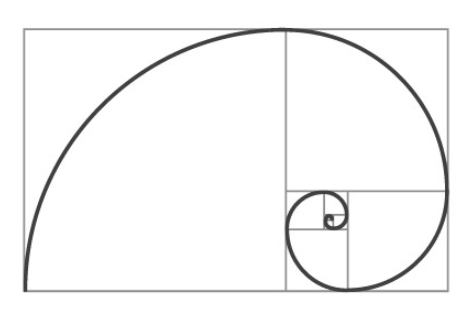
\includegraphics[scale=0.35]{images/golden-ratio.png}
\end{center}

None of these representations, however, really give any reason as to why the golden ratio is so interesting. Here’s an example that starts to be more interesting.

The Fibonacci Sequence, where the $n$th term is denoted as $F_n$, is a sequence of numbers where each number is the sum of the two numbers before it. Mathematicians frequently start the sequence by defining $F_0=0$ and $F_1=1$, and the sequence therefore continues with $1$, $2$, $3$, $5$, $8$, $13$, etc. A natural question is then: is there some closed-form formula for the $n$th term of the sequence?

The answer is Binet’s Formula. Binet’s Formula, out of nowhere, has a fascinating connection to the golden ratio: the $n$th term of the Fibonacci Sequence, $F_n$, is $\frac{\phi^n - \psi^n}{\sqrt5}$, where $\phi$ is the golden ratio and $\psi$ the conjugate of the golden ratio, $\frac{1-\sqrt{5}}{2}$. The Fibonacci Numbers, which is a sequence of integers, not only has a closed-form formula with irrationals, but the golden ratio, out of all numbers!

Another natural question that follows the definition of the Fibonacci Numbers is: how do the numbers behave as the sequence progresses further and further? One way we can quantify this is to find how the ratio between consecutive Fibonacci Numbers changes along the sequence. This is written as $\lim_{n\to\infty}\frac{F_{n+1}}{F_n}$ (read as ``the limit of $\frac{F_{n+1}}{F_n}$ as $n$ approaches infinity''). As the index of the Fibonacci Numbers increases, what number does the ratio between consecutive Fibonacci Numbers approach?
To compute this, we can use a neat trick: we know that $\lim_{n\to\infty}\frac{F_{n+1}}{F_n}=\lim_{n\to\infty}\frac{F_n}{F_{n-1}}$. We can therefore write an equation to find that quantity using the definition of the Fibonacci Numbers: $F_{n+1}=F_n+F_{n-1}$. Letting $x=\lim_{n\to\infty}\frac{F_{n+1}}{F_n}$, we have:

{\footnotesize\begin{align*}
    F_{n+1}&=F_n+F_{n-1}\\
    \frac{F_{n+1}}{F_n}&=\frac{F_n}{F_n}+\frac{F_{n-1}}{F_n}\\
    \frac{F_{n+1}}{F_n}&=1+\frac{1}{\frac{F_n}{F_{n-1}}}\\
    \lim_{n\rightarrow\infty} \frac{F_{n+1}}{F_n}&=1+\frac{1}{\lim_{n\rightarrow\infty} \frac{F_{n}}{F_{n-1}}}\\
    x&=1+\frac{1}{x}\\
    x^2&-x-1=0.
\end{align*}}


But this is exactly one of the definitions of the golden ratio: a solution to the quadratic equation $x^2-x-1=0$ (the second solution is negative, which clearly cannot be the ratio of two positive Fibonacci Numbers)! This means that the ratio of two consecutive Fibonacci Numbers tends to the golden ratio as the sequence progresses, yet another surprising connection between the Fibonacci Numbers and the golden ratio.

However, the golden ratio isn’t just interesting in algebra. It also comes up in surprising situations in geometry, as well. Let’s look at an example problem.

Suppose that we have a regular decagon: a polygon with $10$ sides that all have equal length. Now, let’s take its circumcircle: draw a circle going through all 10 vertices of the polygon. What is the ratio between the radius of the circumcircle of the decagon and the length of a side of the decagon?

\begin{center}
    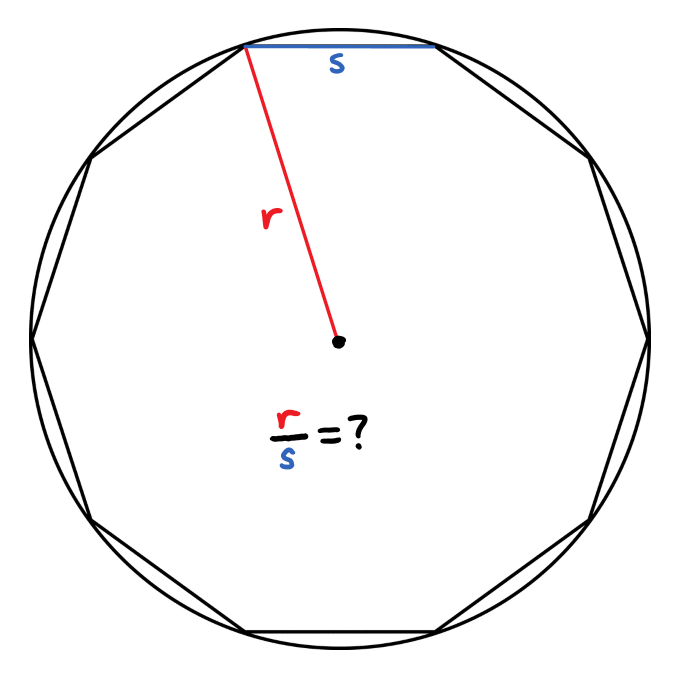
\includegraphics[scale=0.25]{images/golden-ratio3.png}
\end{center}

Let’s suppose that the center of the circumcircle is the point $O$. Then, note that we can create a right triangle by dropping an altitude from $O$ to the midpoint of the side. We then have a right triangle with hypotenuse $r$ and leg $\frac s2$.

\begin{center}
   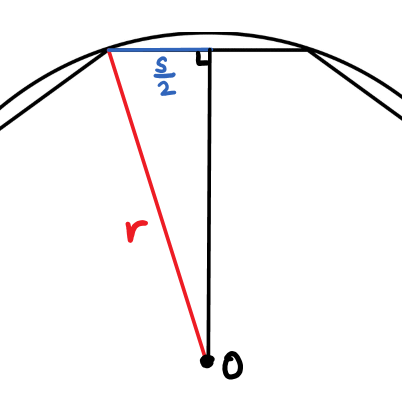
\includegraphics[scale=0.35]{images/golden-ratio4.png}
\end{center}

If we find the ratio between $r$ and $\frac{s}{2}$, we know the ratio between $r$ and $s$. To find $\frac{r}{s/2}$, notice that it is equal to the reciprocal of the $\sin$ of the angle at $O$, as $\sin$ is opposite over hypotenuse! Therefore, we must simply find how large the angle at $O$ is.

We can find the angle at $O$ by cleverly using symmetry: notice that the angle we want is just $\frac1{20}$ of the entire circle, which is $18^\circ$.

\begin{center}
    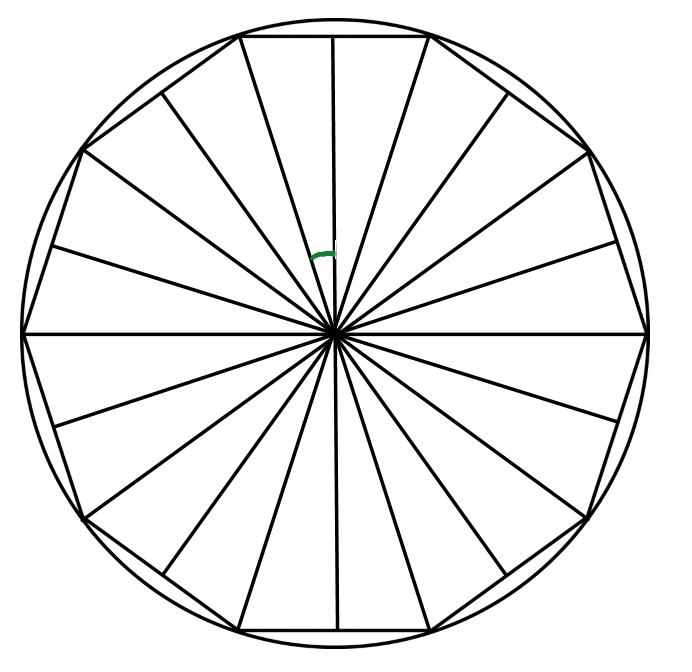
\includegraphics[scale=0.25]{images/golden-ratio5.png}
\end{center}

Therefore, we know that $\frac{r}{s/2} = \frac1{\sin 18^\circ}$, so $\frac rs = \frac1{2\sin 18^\circ}$. What is the value of $\sin 18^\circ$? There are various ways to calculate this\footnote{You can read about them \href{https://math.stackexchange.com/questions/2140356/various-methods-to-find-value-of-sin-18-circ}{here}.}, but once we do, we find that $\sin 18^\circ = \frac{\sqrt5-1}4$. Therefore, we know that $\frac rs = \frac1{2\frac{\sqrt5-1}4} = \frac{\sqrt5+1}2$, exactly the golden ratio!

In sum, the golden ratio is fascinating in mathematics simply due to its ubiquity: why is such an arbitrary number so universally found and used? So, the next time the number $\frac{1+\sqrt5}2$ shows up in a problem, take a brief pause to appreciate the strange appearance of the golden ratio.
\end{document}